
%----------------------------------------------------------------------------------------
%	PACKAGES AND OTHER DOCUMENT CONFIGURATIONS
%----------------------------------------------------------------------------------------

\documentclass[12pt]{article} % Default font size is 12pt, it can be changed here

\usepackage[utf8]{inputenc}

\usepackage{geometry} % Required to change the page size to A4
\geometry{a4paper} % Set the page size to be A4 as opposed to the default US Letter

\usepackage{graphicx} % Required for including pictures

\usepackage{float} % Allows putting an [H] in \begin{figure} to specify the exact location of the figure
\usepackage{wrapfig} % Allows in-line images such as the example fish picture

\usepackage{lipsum} % Used for inserting dummy 'Lorem ipsum' text into the template

\usepackage[shortlabels]{enumitem}
                    
\usepackage{xcolor}

% text-marker-like highlighting of text
% https://tex.stackexchange.com/questions/141569/highlight-textcolor-and-boldface-simultaneously#141572
\usepackage{soulutf8}

\usepackage{hyperref}

% e.g. for user scenario formatting
% https://www.sharelatex.com/learn/Typesetting_quotations
\usepackage{csquotes}

\usepackage{glossaries}
\makeglossaries

\linespread{1.2} % Line spacing

\setlength\parindent{0em} % Uncomment to remove all indentation from paragraphs

\setlength{\parskip}{1.25ex}

\graphicspath{{Pictures/}} % Specifies the directory where pictures are stored


% enumerate list with less spacing
% usage:
% \begin{cptenumerate}
% 	\advantageit Is a very good one
% 	\disadvantageit Is a very, very complex one.
% \end{cptenumerate}
\newenvironment{cptenumerate}[1][label=\arabic*.]{\begin{enumerate}[#1] \setlength\itemsep{0em}}{\end{enumerate}}

\newenvironment{cptitemize}[1][,]{\begin{itemize} \setlength\itemsep{0em}}{\end{itemize}}

\usepackage{cleveref}

\begin{document}

\newenvironment{absolutelynopagebreak}
  {\par\nobreak\vfil\penalty0\vfilneg
   \vtop\bgroup}
  {\par\xdef\tpd{\the\prevdepth}\egroup
   \prevdepth=\tpd}

% https://tex.stackexchange.com/questions/128605/enumitem-referencing-items-in-enumerate
% 1 -- shortname
% 2 -- Funktion
% 3 -- Beschreibung
% 4 -- Quelle
% 5 -- Abhängigkeiten
\newcommand{\req}[5]{%
	\begin{absolutelynopagebreak}
	\item % this is a list item
	\label{#1} % set shortname as label for references
	\textsf{#1} \\ % print shortname
	\textbf{Funktion:} #2 \\
	\textbf{Beschreibung:} #3 \\
	\textbf{Quelle:} #4 \\
	\textbf{Abhängigkeiten:} #5 \\
	\end{absolutelynopagebreak}
}

\newlist{requirements}{enumerate}{100}
\setlist[requirements]{itemsep=-1em}
\newlist{optrequirements}{enumerate}{100}


% Usage:
% \begin{requirements}[ref={(R\arabic*)},label=(R\arabic*)]
%  	 \req{shortname}{foo}{bar}{baz}{qux} 
%  	 \req{myreq}{a}{b}{\ref{shortname}}{d}
%  	 	\req{SpeicherungMovebankNutzerdaten}{
% 		Nutzerdaten für die Movebank sollen in den Einstellungen eingetragen werden können. 
% 		}{
% 		Die App soll in den Einstellungen eine Möglichkeit anbieten, Movebank-Nutzerdaten eintragen zu können, um auch Daten aus der Movebank zu laden, die nur mit einem dortigen Account abrufbar sind. 
% 		}{
% 		Treffen am 26.04.2018 
% 		}{
% 		\ref{DatenLadenAusMovebank}
% 		}
% \end{requirements} 
% Ich beziehe mich auf \ref{shortname} bla bla. Und hier auf \ref{myreq}.

% \begin{optrequirements}[ref={(O\arabic*)},label=(O\arabic*)]
%  	 \req{opta}{foo}{bar}{baz}{qux} 
%  	 \req{optb}{a}{b}{c}{d}
% \end{optrequirements} 
% Ich beziehe mich auf \ref{opta} bla bla. Und hier auf \ref{optb}.


\setlist[enumerate, 1]{1\textsuperscript{o}}

\begin{titlepage}

\newcommand{\HRule}{\rule{\linewidth}{0.5mm}} % Defines a new command for the horizontal lines, change thickness here

\center % Center everything on the page

\textsc{\Large Position Prediction based on Movement Data}\\[0.5cm] % Major heading such as course name
\textsc{\large Software Requirements Specification}\\[0.5cm] % Minor heading such as course title

\vfill

\emph{Autoren}\\
Timo Jockers, Oliver Mänder, Benjamin Moser,\\Manuel Prinz, Sebastian Strumbelj, Simon Suckut

\vfill % Fill the rest of the page with whitespace

\end{titlepage}

%================================================================================================================

\tableofcontents % Include a table of contents

\newpage

%================================================================================================================

\section{Einleitung} \label{einleitung}


\subsection{Überblick}

% Explain, how your document will proceed. (Tell them, what
% you will tell them).
Dieses Dokument ist in fünf Abschnitte aufgeteilt. Im ersten Abschnitt (Kapitel \ref{einleitung}) wird der Zweck dieses Dokuments erläutert und der Funktionsumfang der Applikation grob beschrieben. Desweiteren werden verwendete Definitionen und Abkürzungen sowie weitere referenzierte Dokumente aufgeführt. Im zweiten Abschnitt (Kapitel \ref{kontext}) wird der Kontext beschrieben, in dem das Produkt verwendet werden soll. Darunter fallen das Verhältnis zu anderen Produkten, die Nutzercharakteristika sowie mögliche Abhängigkeiten und Einschränkungen.
Der dritte Abschnitt (Kapitel \ref{mindestanforderungen} bis \ref{nicht-anforderungen}) enthält eine detaillierte Auflistung der Anforderungen. Im vierten Abschnitt (Kapitel \ref{zeitplan}) wird der Projektzeitplan, insbesondere die Meilensteine, festgelegt. Der letzte Abschnitt (Kapitel \ref{diagramme}) enthält die wesentlichen UML-Diagramme.
%------------------------------------------------

\subsection{Zweck dieses Dokumentes}


% Why do we write an SRS?
% Whom do we write this document for?

 Dieses Dokument dient  zur Fixierung der erhobenen Anforderungen und Einschränkungen an die zu entwickelnde Applikation. Damit liefert es eine Grundlage und Referenz für den Entwicklungsprozess sowie für die Überprüfung des Systems auf Vollständigkeit nach Fertigstellung. Für den Kunden legt dieses Dokument fest, welcher Funktionsumfang realisiert werden wird.

%------------------------------------------------

% "Scope"
\subsection{Produktbeschreibung}

% State the product to be produced
% Take care to make this consistent with other documents.
Die zu entwickelnde Android-Applikation trifft, basierend auf Informationen aus der Vergangenheit, eine Vorhersage über den Aufenthaltsort eines Vogels zu einem gegebenen Zeitpunkt in der Zukunft. 

Dabei kann der Nutzer wählen, welche der verfügbaren Daten und Verfahren in die Vorhersage einfließen. 

Das Ergebnis der Vorhersage wird in einer zwei- oder dreidimensionalen Kartenlandschaft visualisiert.

% \hl{Weiterhin ist integriert eine VR-Visualisierung. (Zu klären!)}


\subsection{Definitionen und Abkürzungen}

% Könnte man machen, evtl. zu Umständlich
% \newglossaryentry{forscher}{name=Forscher, description={%
% 	Ein Mitarbeiter des Max-Planck-Instituts und Nutzer der App.
% }}

% \newglossaryentry{utc}{name=UTC, description={Coordinated Universal Time}}
% \newglossaryentry{adt}{name=ADT, description={Atlantic Daylight Time}}
% \newglossaryentry{est}{name=EST, description={Eastern Standard Time}}

% \printglossaries
 
% % Use the terms
% \gls{utc} is 3 hours behind \gls{adt} and 10 hours ahead of \gls{est}.

\paragraph{App, Applikation} Soweit nicht anders angemerkt wird hiermit die zu entwickelnde Android-Applikation bezeichnet.
 \paragraph{Forscher} Personen, die wissenschaftlich das Verhalten von Vögeln untersuchen.
 \paragraph{Mobile Daten} Ein Smartphone kann sich entweder über ein WiFi-Netzwerk oder über ein mobiles Datennetzwerk (3G, LTE, ...) mit dem Internet verbinden. 
\paragraph{Vorhersage-Modell/Algorithmus} Die zur Berechnung einer Vorhersage verwendete Methodik. 
\paragraph{API} \textit{Application Programming Interface}, hier insbesondere Schnittstellen mit Providern wie \textit{Movebank} oder \textit{Cesium}. 
\paragraph{Outdoor-Modus, Normal-Modus} Die Applikation verfügt über zwei verschiedene Funktionsmodi. Einer davon ist der sog. Outdoor-Modus. (Siehe Anforderung \ref{Modi}.)
\paragraph{Cesium} Ist eine Javascript-Bibliothek für die Arbeit mit dreidimensionalen Kartendaten.
\paragraph{Offline-Karten} Ist ein 2D-Karten-Provider der Kartendaten liefert, wenn keine Internetverbindung besteht.

\subsection{Referenzen}

\begin{itemize} 
 	 \item  \href{https://docs.google.com/document/d/1Yc2f18JFaHyhrgM2h2WiATQ0zVmZnsc9W1ImhwWJF-g/edit?usp=sharing}{Begleitdokument zum Softwareprojekt SS 2018}
 	 \item \href{https://cesiumjs.org/refdoc/}{Cesium API-Dokumentation}
\end{itemize} 



%================================================================================================================

\newpage
\section{Produktkontext} \label{kontext}

\subsection{Externe Produkte}
% Relation to other products (e.g. overall system ⇒ Class diagram?)
% • Known interfaces (e.g. Mailserver)
Die Applikation soll Forschern eine Vorhersage bieten können, wo sie einen Vogel mit einer gewissen Wahrscheinlichkeit in naher Zukunft antreffen werden. 

In der Vergangenheit aufgezeichnete Positionsdaten werden dabei von \textit{Movebank} bezogen. Das Ergebnis der Vorhersage wird mittels \textit{Cesium} und \textit{Offline-Karten} visualisiert.


% User Characteristics
\subsection{Nutzercharakterisierung}

Die Nutzer der Applikation sind Forscher, die das Verhalten von Vögeln untersuchen.

Der Nutzer verfügt über mindestens gute Erfahrung im Umgang mit Smartphones und deren Bedienung.

Der Nutzer hat im Allgemeinen eine Vorstellung vom Umfang der verwendeten Datenmengen, der Komplexität der Analyse und ist sich bewusst, dass entsprechende Ergebnisse - je nach Gerät und technischen Voraussetzungen - mehrere Sekunden dauern können.

Der Nutzer hat Erfahrung im Umgang mit geographischen Daten. Er kennt grundlegende Visualisierungstechniken und deren Interpretation. 


\subsection{Szenario}

Der folgende Text beschreibt beispielhaft ein Szenario, wie die Applikation verwendet wird.

\begin{displayquote}
\small
Herr Herr Storch ist ein Forscher am Max-Planck-Institut für Ornithologie. Herr Storch beschäftigt sich mit der Analyse von Tracking-Daten von Vögeln. Für das Tracking werden Vögel mit Sendern ausgestattet. 

Herr Storch möchte nun einen bestimmten in der Vergangenheit über einen solchen Sender verfolgten Vogel nun wieder auffinden, etwa um den Sender auszutauschen oder um das Tier zu betrachten.

Herr Storch befindet sich in seinem Büro und hat Zugriff auf eine schnelle Datenverbindung. Herr Storch startet die Applikation auf seinem Smartphone im Normal-Modus und gibt die Vogel-ID ein. Er benötigt noch etwas Zeit zur Vorbereitung und für das Zurücklegen des Weges, also fragt er eine Vorhersage für eine dreiviertelstunde in der Zukunft an.

Die Vorhersage wird Herr Storch in der \textit{Cesium}-Umgebung visualisiert. Es wird ein Bereich angezeigt, in dem der Vogel mit hoher Wahrscheinlichkeit anzutreffen ist sowie weitere Abstufungen die einer geringeren Wahrscheinlichkeit entsprechen. Mithilfe der dreidimensionalen Kartendarstellung macht sich Herr Storch außerdem mit der Beschaffenheit des Geländes vertraut. Währenddessen speichert die Applikation die Daten der Vorhersage und 2D-Kartendaten für spätere Verwendung.

Nun bricht Herr Storch auf. Da das Gebiet recht abgelegen ist verfügt sein Smartphone lediglich über eine langsame mobile Datenverbindung und an manchen Stellen über gar keine Internetverbindung. Herr Storch wechselt nun in den Outdoor-Modus. Die Applikation greift nun zur Visualisierung der Vorhersage auf die vorher heruntergeladenen 2D-Karten zurück.

Die aktuelle Position von Herr Storch wird mittels des GPS-Sensors seines Smartphones ebenfalls in der Visualisierung angezeigt. Damit nähert sich Herr Storch dem Zielgebiet an und wird bei der Vogelsuche unterstützt.
\end{displayquote}


\subsection{Annahmen und Abhängigkeiten}

% \begin{itemize} 
%  	 \item vorhersage-modelle
%  	 \item datenbank vorhanden
%  	 \item movebank erreichbar 
%  	 \item vogel-id/name vorhanden
% \end{itemize} 

\begin{itemize} 
 	 \item Die verwendeten Schnittstellen (\textit{Movebank}, \textit{Cesium}, ...) sind zu jedem Zeitpunkt verfügbar.
 	 \item \hl{Eine für die Abfrage der Daten aus \textit{Movebank} ausreichende Identifikation des gesuchten Vogels ist vorhanden.}
 	 \item Werden für die Datenabfrage aus \textit{Movebank} weitere Schritte oder Informationen benötigt (Zugangsdaten, vorherige Anfrage bei Provider der Daten, ...) so werden diese vom Nutzer erledigt bzw. bereitgestellt.
 	 \item Es wird bis zu Milestone 2 ein rudimentäres Vorhersagemodell auf Basis von Positionsdaten aus der Vergangenheit implementiert. Im Laufe der Entwicklung wird in Absprache mit Betreuuern und Kunde ermittelt, welche weiteren Daten und welche weiteren Vorhersagemodelle sinnvoll einbezogen werden können.
\end{itemize} 

% Any other things, that have to be mentioned (e.g. external
% schemata or similar).

\subsection{Einschränkungen}
% Things that could constraint the development
% • Law, Company internals, hardware limitations, safety
% criticality, ...

\begin{itemize} 
	\item Die Applikation soll unter einer Open-Source-Lizenz entwickelt werden. Wird Code oder werden Bibliotheken von Dritten verwendet, so müssen die Lizenzen kompatibel sein.
	\item Die Abfrage von Daten von Schnittstellen kann limitiert sein.
	\item Die Internetverbindung des Gerätes kann während der Nutzung für kurze oder längere Zeit ausfallen.
	\item Bei Verwendung des mobilen Datennetzes kann nur eine kleine Übertragungsgeschwindkeit verfügbar sein.
	\item Von \textit{Movebank} bezogene Daten können unvollständig oder falsch formatiert sein.
	\item Die Software soll aus Modulen aufgebaut werden. Diese Module sollen möglichst unabhängig voneinander sein.
	\item Der Programmcode soll kommentiert und dokumentiert werden.
\end{itemize} 

% The system shall adhere to known standards and built systems and be
% strictly on budget (TODO: Reference to "no fancy new expensive stuff").
% \noindent
% The system shall always enforce the wealth of the animal beings.


%================================================================================================================

\newpage
\section{Mindestanforderungen} \label{mindestanforderungen}

% class diagram, use case diagram, seq diag

\subsection{Funktionen}

\subsubsection{Datenmanagement}

\begin{requirements}[ref={(R\arabic*)},label=(R\arabic*)]
\req{DatenLadenAusMovebank}{
Daten sollen aus der Movebank geladen werden. 
}{
Das Laden der für die Berechnung benötigten Daten geschieht ausschließlich über die Movebank, die die gegeben Daten zur Verfügung stellt. 
}{
Treffen am 26.04.2018 
}{
- 
}
\req{SpeicherungMovebankNutzerdaten}{
Nutzerdaten für die Movebank sollen in den Einstellungen eingetragen werden können. 
}{
Die App soll in den Einstellungen eine Möglichkeit anbieten, Movebank-Nutzerdaten eintragen zu können, um auch Daten aus der Movebank zu laden, die nur mit einem dortigen Account abrufbar sind. 
}{
Treffen am 26.04.2018 
}{
\ref{DatenLadenAusMovebank}
}
\req{OfflineDatenSpeicherung}{
Die App soll für die aktuelle Vorhersage Offline-Daten speichern. 
}{
Die App soll die aktuelle Vorhersage lokal speichern, damit man diese auch ohne aktiven Internetzugang betrachten kann. 
}{
Treffen am 26.04.2018 
}{
\ref{BerechnungDesAufenthaltsraumes}
}
\req{AktualisierungUeberMobileDaten}{
Über mobile Daten soll die aktuelle Vorhersage aktualisiert werden können. 
}{
Die App soll auch über mobile Daten aktuelle Daten aus der Movebank empfangen und für eine aktuelle Vorhersage verwenden können. 
}{
Treffen am 30.04.2018 
}{
\ref{VisuelleDarstellungDerVorhersage}, \ref{DatenLadenAusMovebank}, \ref{VisualisierungDerVorhandenenDaten}, \ref{BerechnungDesAufenthaltsraumes}, \ref{VorhersageFuerBestimmtenZeitraum}, \ref{VisualisierungBeiOutdoorModus} 
}
\end{requirements}

\subsubsection{Vorhersageberechnung}

\begin{requirements}[ref={(R\arabic*)},label=(R\arabic*),resume]
\req{BerechnungDesAufenthaltsraumes}{
 Gegeben die StudyID und VogelID soll ein wahrscheinlicher Aufenthaltsraum berechnet werden. 
 }{
 Für einen Vogel (und Study??) soll berechnet wie wahrscheinlich es ist, diesen in einem vom Algorithmus bestimmten Gebiet anzutreffen. 
 }{
 Treffen am 26.04.2018 
 }{
 \ref{DatenLadenAusMovebank} 
}
\req{VorhersageFuerBestimmtenZeitraum}
{
 Die Positionsvorhersage soll für einen gegebenen Zeitraum berechnet werden. 
 }{
 Die Positionsvorhersage soll für einen gegeben Zeitraum ab dem aktuellen Moment berechnet werden. 
 }{
 Treffen am 26.04.2018 
 }{
 \ref{DatenLadenAusMovebank} 
}
\req{WaehlbarerVorhersagezeitraum}
{
 Der Nutzer soll den Zeitraum für die Vorhersage wählen können.
 }{
 Der Nutzer soll die Möglichkeit haben, einzustellen für welchen Zeitraum ab dem aktuellen Zeitpunkt die Vorhersage berechnet wird. 
 }{
 Treffen am 26.04.2018
 }{
 - 
}
\req{WahlDerDatenFuerVorhersage}
{
 Der Nutzer soll einstellen können auf welchen Daten die Vorhersage basiert.
 }{
 Der Nutzer soll über Parameter die Berechung der Vorhersage justieren können.}{
 Treffen am 26.04.2018
 }{
 \ref{DatenLadenAusMovebank} 
}
\end{requirements}

\subsubsection{Visualisierung}

\begin{requirements}[ref={(R\arabic*)},label=(R\arabic*),resume]
\req{VisuelleDarstellungDerVorhersage}
{
 Die Vorhersagen sollen visuell dargestellt werden. 
 }{
 Die Berechnungen zur Vorhersage der wahrscheinlichen Vogelposition sollen in der App angezeigt werden. 
 }{
 Treffen am 26.04.2018 
 }{
 \ref{DatenLadenAusMovebank} 
}
\req{Kompass}
{
 Es soll ein Kompass angezeigt werden, der zum gesuchten Vogel zeigt. 
 }{
 Eine Visualisierung soll anzeigen, in welcher Richtung ausgehend vom aktuellen Standpunkt der gesuchte Vogel am wahrscheinlichsten anzutreffen ist. 
 }{
 Treffen am 02.05.2018 
 }{
 \ref{DatenLadenAusMovebank} 
}
\req{AktuellePosition}
{
 Es soll die aktuelle Position angezeigt werden. 
 }{
 Eine Visualisierung soll auf der dargestellten Kartenlandschaft anzeigen, wo sich der Nutzer momentan befindet.
 }{
 Treffen am 02.04.2018 
 }{
 \ref{VisualisierungInCesiumBeiNormalModus}, \ref{VisualisierungInBeiOutdoorModus} 
}
\req{VisualisierungDerVorhandenenDaten}
{
 Die vorhandenen Daten für einen gegebenen Vogel und Zeitraum sollen visualisiert werden. 
 }{
 Wird ein Vogel ausgewählt, so sollen dessen vorhandene Daten bis zu einer gewählten maximalen Zeitgrenze in der Vergangenheit angezeigt werden können.
 }{
 Treffen am 26.04.2018 
 }{
 \ref{DatenLadenAusMovebank} 
}
\req{VisualisierungInCesiumBeiNormalModus}
{
 Im Normal-Modus sollen die Daten in Cesium visualisiert werden.
 }{
 Befindet sich die Applikation im Normal-Modus, so sollen die getrackten Positionen und die Vorhersagen mit Cesium visualisiert werden.
 }{
 Treffen am 26.04.2018
 }{
 \ref{DatenLadenAusMovebank}, \ref{VisualisierungDerVorhandenenDaten}, \ref{BerechnungDesAufenthaltsraumes}, \ref{VorhersageFuerBestimmtenZeitraum}
}
\req{VisualisierungBeiOutdoorModus}
{
 Im Outdoor-Modus sollen die Daten visualisiert werden.
 }{
 Befindet sich die Applikation im Outdoor-Modus, so sollen die getrackten Positionen und die Vorhersagen visualisiert werden.
 }{
 Treffen am 30.04.2018
 }{
 \ref{DatenLadenAusMovebank}, \ref{VisualisierungDerVorhandenenDaten}, \ref{BerechnungDesAufenthaltsraumes}, \ref{VorhersageFuerBestimmtenZeitraum}
}
\req{VisualisierungAufOfflineKarten}
{
 Im Outdoor-Modus sollen die Daten auf offline-Karten visualisiert werden.
 }{
 Falls offline-Karten vorhanden sind, sollen diese für die Visualisierung der Vorhersage und der getrackten Positionen verwendet werden. 
 }{
 Treffen am 30.04.2018
 }{
 \ref{DatenLadenAusMovebank}, \ref{VisualisierungDerVorhandenenDaten}, \ref{BerechnungDesAufenthaltsraumes}, \ref{VorhersageFuerBestimmtenZeitraum}
}
\end{requirements}

\subsubsection{Nutzerinteraktion}

\begin{requirements}[ref={(R\arabic*)},label=(R\arabic*),resume]
\req{Modi}
{
 Die Applikation soll über einen Normal- und einen Outdoor-Modus verfügen. 
 }{
 Die Applikation soll über zwei Modi bzw. Zustände verfügen mit ähnlichem aber ungleichem User Interface und Funktionalität. 
 }{
 Treffen am 02.05.
 }{
 - 
}
\req{WechselDesModus}
{
 Der Nutzer soll zwischen dem Normal- und dem Outdoor-Modus wechseln können. 
 }{
 Der Nutzer soll durch Bedienung des User Interfaces zwischen dem Normal und dem Outdoor-Modus wechseln können. 
 }{
 Treffen am 02.05 
 }{
 \ref{Modi} 
}
\req{TouchBasierteBenutzeroberflaeche}
{
 Die App soll über eine touch-basierte Benutzeroberfläche verfügen. 
 }{
 Die App soll über eine touch-basierte Benutzeroberfläche bedienbar sein. 
 }{
 Treffen am 26.04.2018 
 }{
 - 
}
\req{SucheNachVogel}
{
 In der Software soll nach einem Vogel mittels seiner VogelID gesucht werden können.
 }{
 Der Benutzer soll anhand einer ID nach einem bestimmten Vogel suchen können.
 }{
 Treffen am 26.04.2018
 }{
 -
}
\req{HinweisAufFormalFalscheDaten}
{
 Der Nutzer soll auf einen hohen Anteil falsch formatierter Daten hingewiesen werden. 
 }{
 Die App soll dem Nutzer einen Hinweis anzeigen, wenn in den der Berechnung der Vorhersage zugrunde liegenden Daten so viele Datensätze falsch formatiert sind, dass die Qualität der Vorhersage nicht vergleichar mit der auf Basis eines vollständig korrekten Datensatzes ist.
 }{
 Treffen am 30.04.2018 
 }{
 \ref{DatenLadenAusMovebank} 
}
\end{requirements}

\subsection{Nicht-funktionale Anforderungen}

\subsubsection{Hardware}

\begin{requirements}[ref={(R\arabic*)},label=(R\arabic*),resume]
\req{KorrekteArchitekturDerSmartphones}
{
 Die App sollte auf Smartphones mit Android 5.1 oder höher, Internet-Zugang und einer armeabi, armeabi-v7a oder arm64-v8a Architektur lauffähig sein. 
 }{
 Die App sollte auf Smartphones mit Android 5.1 oder höher, Internet-Zugang und einer armeabi, armeabi-v7a oder arm64-v8a Architektur lauffähig sein. 
 }{
 Treffen am 30.04.2018 
 }{
 - 
}
\end{requirements}

\subsubsection{Implementierung}

\begin{requirements}[ref={(R\arabic*)},label=(R\arabic*),resume]
\req{EinheitlicheSchnittstelleFuerVorhersagealgorithmen}
{
 Die Software soll über eine einheitliche Schnittstelle für Vorhersagealgorithmen verfügen.
 }{
 Zum einfachen Hinzufügen von weiteren Vorhersagealgorithmen soll die Software über ein einheitliches Interface für diese verfügen.
 }{
 Treffen am 26.04.2018
 }{
 -
}
\end{requirements}

\subsubsection{Robustheit}

\begin{requirements}[ref={(R\arabic*)},label=(R\arabic*),resume]
\req{VerhaltenOhneInternetverbindung}
{
 Die App sollte bei fehlender Internetverbindung mit eingeschränkter Funktionalität weiter nutzbar sein. 
 }{
 Bricht die Verbindung zum Internet ab, sollte die App robust darauf reagieren. Einige Grundfunktionen sollten dabei weiter nutzbar sein. 
 }{
 Treffen am 30.04.2018 
 }{
 - 
}
\req{RobustGegenueberFormalFalschenDaten}
{
 Die App soll robust gegenüber formal falschen Daten aus der Movebank sein 
 }{
 Die App soll formal falsche Daten, die sie aus der Movebank bekommt, so aufbereiten, dass das Berechnen und Visualisieren eines Ergebnisses möglich ist. 
 }{
 Treffen am 26.04.2018 
 }{
 \ref{DatenLadenAusMovebank} 
}
\end{requirements}

\subsubsection{Performanz}

\begin{requirements}[ref={(R\arabic*)},label=(R\arabic*),resume]

\req{BerechnungsdauerVorhersage}
{
 Der Berechnungsdauer der Vorhersage soll die vom Nutzer erwartete Dauer nicht deutlich überschreiten. 
 }{
 Die App soll die Vorhersage in einem adäquaten Zeitraum berechnen und diese dem Nutzer möglichst schnell visualisieren. 
 }{
 Treffen am 30.04.2018 
 }{
 \ref{VisuelleDarstellungDerVorhersage}, \ref{DatenLadenAusMovebank}, \ref{VisualisierungDerVorhandenenDaten}, \ref{BerechnungDesAufenthaltsraumes}, \ref{VorhersageFuerBestimmtenZeitraum}, \ref{WahlDerDatenFuerVorhersage}, \ref{RobustGegenueberFormalFalschenDaten} 
}

\end{requirements}
 \section{Optionale Anforderungen} \label{optionale_anforderungen}

 Die folgenden Anforderungen sind optional und müssen nicht zwingend erfüllt werden.

\begin{requirements}[ref={(O\arabic*)},label=(O\arabic*)]
\req{VirtualReality}
{
 Integration von \textit{Virtual Reality}-Umgebung
 }{
 Es wird ein zur Verfügung gestelltes Modul in die Applikation integriert, dass die Visualisierungen in einem \textit{Virtual Reality}-Raum visualisiert. 
 }{
 Treffen am 26.04.2018 
 }{
 - 
}

\req{ZusaetzlicheParameter}
{
 Es werden - neben den Positionsdaten aus der Vergangenheit - noch weitere Parameter für die Berechnung der Vorhersage verwendet. 
 }{
 Weitere Parameter / Datenquellen fließen in die Berechnung der Vorhersage ein. Zum Beispiel kann das Wetter oder ähnliche Attribute mit zur Berechnung benutzt werden.
 }{
 Begleitdokument 
 }{
 - 
}

\req{GewichtungParameter}
{
 Parameter, die in die Berechnung der Vorhersage einfließen sollen gewichtet werden können. 
 }{
 Der Nutzer soll die Möglichkeit haben einzustellen, mit welchem Gewicht die jeweiligen Parameter in die Berechnung der Vorhersage einfließen.
 }{
 Begleitdokument 
 }{
 \ref{BerechnungDesAufenthaltsraumes} 
}

\req{VariableDarstellung}
{
 Es sind verschiedene Arten der Visualisierung verfügbar. 
 }{
 Der Nutzer hat die Möglichkeit, das Ergebnis der Vorhersage auf verschiedene Arten zu visualisieren. 
 }{
 Begleitdokument 
 }{
 \ref{BerechnungDesAufenthaltsraumes}, \ref{VisuelleDarstellungDerVorhersage} 
}

\req{Evaluation}
{
 Eine Evaluation der Vorhersage ist möglich. 
 }{
 Der Nutzer hat die Möglichkeit, das Ergebnis der Vorhersage zu bewerten. 
 }{
 Begleitdokument 
 }{
 \ref{BerechnungDesAufenthaltsraumes} 
}

\req{MehrereVoegel}
{
 Es kann eine Vorhersage für mehrere Vögel gemeinsam getroffen und visualisiert werden. 
 }{
 Für eine gegebene Menge von Vögeln kann eine Vorhersage getroffen und eine Visualisierung erstellt werden. 
 }{
 Begleitdokument 
 }{
 \ref{BerechnungDesAufenthaltsraumes}, \ref{VisuelleDarstellungDerVorhersage} 
}

\req{Gattung}
{
 Andere Tiere derselben Gattung werden in die Berechnung der Vorhersage einbezogen. 
 }{
 Es werden die Daten von anderen Tieren derselben Gattung für die Berechnung der Vorhersage eines bestimmten Vogels verwendet. 
 }{
 Begleitdokume
 }{
 \ref{MehrereVoegel}, \ref{ZusaetzlicheParameter} 
}

\req{AehnlichkeitenFinden}{
 Es werden Muster in den Daten aus der Vergangenheit für die Berechnung der Vorhersage verwendet. 
 }{
 Die Analyse von Mustern in Daten aus der Vergangenheit fließt in die Berechnung der Vorhersage ein. 
 }{
 Begleitdokument 
 }{
 \ref{BerechnungDesAufenthaltsraumes}, \ref{ZusaetzlicheParameter} 
}

\end{requirements}




 \section{Nicht-Anforderungen} \label{nicht-anforderungen}

Die App soll lediglich ein einfaches Vorhersageverfahren beinhalten, und zusätzlich eine interne Schnittstelle zur Verfügung stellen, um die vom Kunden zur Verfügung gestellten Modelle/Algorithmen zu integrieren.

Es ist nicht Teil des Entwicklungsprozesses, ein komplexes Vorhersagemodell zu entwickeln.

Es werden keine Vorhersagen für lange Zeiträume (im Maßstab von mehreren Tagen) getroffen.

%================================================================================================================

\newpage
\section{Projektzeitplan} \label{zeitplan}

\subsection*{Milestone 1}
Fertigstellung am 15.5.
\begin{itemize} 
	\item Grundliegende Software-Architektur festgelegt
	\item Grundliegendes Software-Design festgelegt
	\item Ein Grundgerüst der Applikation ist fertiggestellt: Es sind folgende Ansichten funktional umgesetzt:
	\begin{itemize} 
		\item Cesium (eine Kartenumgebung wird angezeigt, Navigation möglich)
		\item Offline-Karten (eine Kartenumgebung wird angezeigt, Navigation möglich)
		\item Diverse UI-Elemente (mindestens Eingabefeld, Button)
	\end{itemize} 
	\item Die Positionsdaten für die Vorhersage werden von der \textit{Movebank}-API bezogen.
\end{itemize} 

\vspace{1em}

\subsection*{Milestone 2}
Fertigstellung am 5.6.
\begin{itemize} 
	\item Es wird eine Vorhersage mittels eines einfachen Vorhersagemodells berechnet.
	\item Es existiert eine funktionale Visualisierung des Vorhersage-Ergebnisses.
	\item Der Aufbau des User-Interfaces ist festgelegt (nicht-funktionale Mockups).
\end{itemize}

\vspace{1em}

\subsection*{Milestone 3}
Fertigstellung am 10.7.
\begin{itemize} 
	\item Anforderungen, die mit eingeschränktem Internetzugriff in Verbindung stehen sind realisiert.
	\item Die momentan angezeigte Vorhersage kann aktualisiert werden (Prüfung, ob neue Daten verfügbar, Neuberechnung; auch unter Verwendung von lediglich mobilem Datennetz)
	\item Die Visualisierung ist vollständig und auf gute Interpretierbarkeit und Ästhetik optimiert.
	\item Das User Interface ist vollständig und auf gute Benutzbarkeit und Ästhetik optimiert.
\end{itemize} 


%================================================================================================================

\newpage
\section{Diagramme} \label{diagramme}

\subsection{Anwendungsfälle}

In folgendem Diagramm sind die wesentlichen Anwendungsfälle der Applikation und ihre Beziehungen dargestellt. Die einzelnen Anwendungsfälle werden im Folgenden detailliert erläutert und eventuell alternative Abläufe beschreiben.

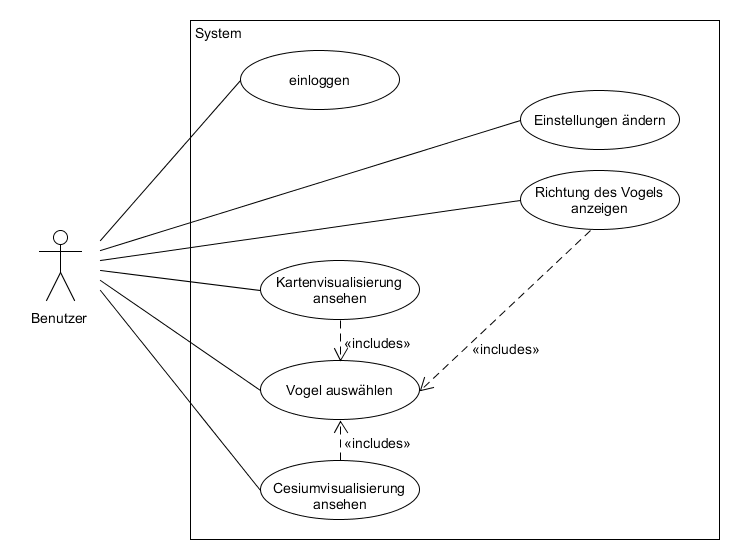
\includegraphics[width = 1\linewidth]{Usecasediagramm.png}

\paragraph{Einloggen} Der Nutzer hat die Möglichkeit, sich bei der \textit{Movebank}-API zu authentifizieren.
\begin{cptenumerate} 
  	 \item Eingabe der Zugangsdaten
  	 \item Übermittlung der Zugangsdaten bei Anfrage an \textit{Movebank}
  	 \begin{cptenumerate}[a.]
  	  	 \item Rückgabe der angefordeten Daten
  	  	 \item Benachrichtigung über fehlgeschlagene Authentifizierung
  	 \end{cptenumerate} 
 \end{cptenumerate}  

 \paragraph{Einstellungen ändern} Der Nutzer hat die Möglichkeit, Einstellungen der Applikation zu ändern.

 \paragraph{Richtung des Vogels anzeigen} Es wird visualisiert, in welcher Richtung - ausgehend vom Nutzer - der Vogel anzutreffen ist.

 \paragraph{Vogel auswählen} Der Nutzer kann einen Vogel anhand seiner ID auswählen.
 \begin{cptenumerate} 
     	 \item Eingabe der ID
     	 \item Abfrage der ID von \textit{Movebank}
     	 \begin{cptenumerate}[a.]
     	   	 \item Weiter zur Visualisierung
     	   	 \item Benachrichtung über fehlerhafte oder nicht gefundene ID
     	  \end{cptenumerate}  
    \end{cptenumerate}    

\paragraph{Kartenvisualisierung ansehen, Cesiumvisualisierung ansehen} Der Nutzer betrachtet die Visualisierung des Ergebnisses der Vorhersage auf einer Kartenlandschaft.
\begin{cptenumerate}[a.]
 	 \item Falls im Normal-Modus: Darstellung in \textit{Cesium}.
 	 \item Falls im Outdoor-Modus: Darstellung mit \textit{Offlinekarten}. 
\end{cptenumerate}


\subsection{Abläufe}

Im folgenden Diagramm wird exemplarisch ein Informationsaustausch zwischen beteiligten Komponenten und dessen zeitlicher Ablauf in einer vollständigen Sitzung des Nutzers illustriert. 

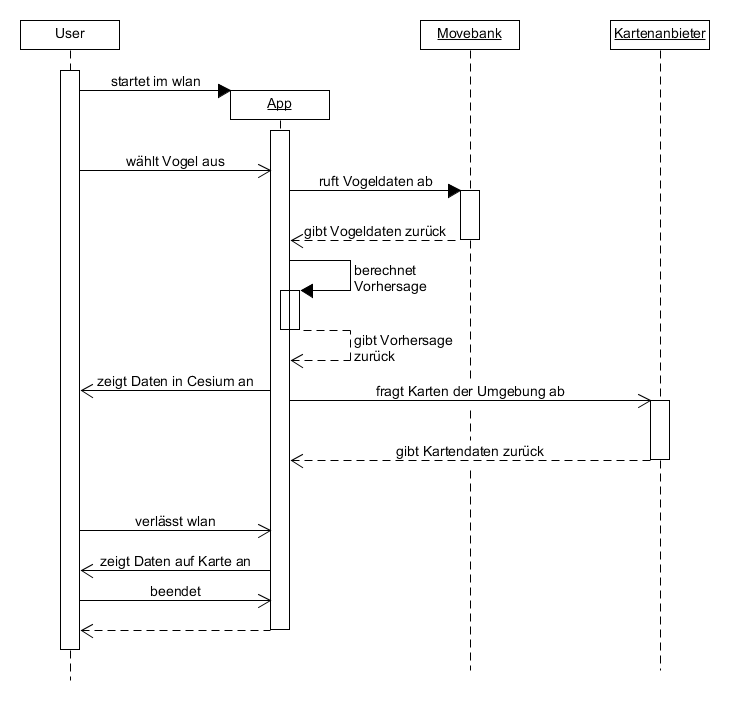
\includegraphics[width = 1\linewidth]{Sequenzdiagramm.png}

\begin{cptenumerate} 
 	 \item Der Nutzer startet die Applikation.
 	 \item Der Nutzer wählt über das User Interface einen Vogel aus.
 	 \item Die Applikation ruft für den spezifizierten Vogel Daten aus \textit{Movebank} ab.
 	 \item Die Applikation berechnet eine Vorhersage.
 	 \item Die Vorhersage wird in \textit{Cesium} visualisiert.
 	 \item Es werden 2D-Kartendaten von einem Kartenanbieter abgefragt und zwischengespeichert.
 	 \item Der Nutzer wechselt in den Outdoor-Modus.
 	 \item Die Vorhersage wird auf einer 2D-Kartenlandschaft visualisert.
 	 \item Die Applikation wird beendet.
\end{cptenumerate} 

\end{document}